\documentclass[a4paper]{report}
\usepackage[english]{babel}
\usepackage{amsfonts}
\usepackage{amsmath} % Equation numbering
\usepackage[square,sort,comma,numbers]{natbib}

\usepackage{graphicx} % Figures
\usepackage{grffile} % For recognising the png-extension
\usepackage{float} % For floating figures

\usepackage{changes} % For track changed extensions
\usepackage{todonotes}

\usepackage{dsfont} % For indicator function

\usepackage{hyperref}
\bibliographystyle{plainnat}

% For example environment
\usepackage{amsthm}
\theoremstyle{definition}
\newtheorem{example}{Example}[section]

% For theorem environment
\newtheorem{theorem}{Theorem}

\begin{document}
\chapter{Comparison of iteration methods}
In this section, the three algorithms for numerically solving the simple discounted problem will be compared.
The algorithms that will be compared are Value Iteration, Policy Improvement and a custom iteration method.
These algorithms were implemented in Matlab.
The algorithms were compared for different lifetime distributions, discounts, costs and starting points.
The hazard rate is assumed to be increasing.
\section{Implementations}
In this section, the implementation details of each iteration algorithm will be provided.
Each algorithm has as input the problem parameters.
These consist of the repair cost $c$, additional corrective repair cost $a$, continuous discount $\beta$ and a lifetime distribution with corresponding cumulative distribution function, probability density function and hazard rate.
\subsection{Value Iteration}
Time is equally discretized into 1001 stages with intervals of 0.01 time units in between.
In the first state, the machine is broken and in the $i$'th state (i>1) the machine has lived a time of $0.01(i-1)$ time units.
If a continuous discount $\beta$ is chosen, the discount factor will be $e^{-0.01\beta}$.
Value iteration takes an initial value function as additional input.
The function outputs a control limit and a value function, this control limit is the first time at which repair was chosen.

\subsection{Policy Improvement}
Policy improvement starts with a control limit $\mu_0$, computes the exact expected total discount cost $V(\mu_0)$ corresponding to this control limit and then tries to improve this by slightly changing this control limit to $\mu_{n+1}=\mu_n+\Delta_n$.
If the policy has not improve,i.e. $V(\mu_n)\leq V(\mu_{n+1})$, then we change the direction and size of the improvements to $\Delta_{n+1}=-\rho\Delta_n$ for some $0<\rho<1$.
Else, we keep $\Delta_{n+1}=\Delta_n$.
In the implementation, $\rho=0.45$ was chosen ($\rho=0.5$ could cause certain control limits to be evaluated twice).
As input, this algorithm requires an initial control limit $\mu_0$.
The algorithm outputs a control limit and a corresponding total discounted cost.

\subsection{Custom Iteration}
The custom iteration method starts with some positive cost $V_0$ and then chooses the optimal control limit assuming $V_0$ as terminal cost.
The resulting cost is then $V_1$.
The optimal control limit is found by finding the $\mu_{n+1}$ that satisfies
$$
h(\mu_{n+1})= \beta\frac{c+V_n}{a}.
$$
As we assume $h$ is increasing, there is at most one solution to this. If there is none,  we choose $\mu_{n+1}=\infty$ resulting in the policy of never repairing preventively.
This will be repeated for each iteration.
This simple iteration method could optionally also be enhanced by updating $V_{n+1}$ to $V(\mu_{n+1})$ instead of approximating it using $V_n$.
This results in faster convergence while it doesn't take much more computation.
This would essentially be a version of policy improvement where the new policy would be chosen in a smart way.
The reason that this is not implemented, is that a similar method would probably not be feasible for more difficult problems.

\section{Comparison}
The iteration methods are compared by the speed of convergence.
The resulting control limit after each iteration will be plotted for each algorithm.
Separately, we will also plot the corresponding cost approximation.

There is a slight mismatch between the inputs and outputs of the algorithms which makes it challenging to compare them.
For example, policy iteration takes an initial control limit as input, value iteration takes an initial value function and the custom iteration takes an initial value as input.
From a given initial control limit, we can derive the corresponding total discounted cost and value function and use these as input.
If we take the total discounted cost $V(\mu_0)$ corresponding to some control limit $\mu_0$, we can calculate the corresponding value function at time $t$
\begin{equation}
V(\mu_0,t)=\begin{cases}
\frac{ e^{\beta t}}{\mathbb{P}(Q>t)} [V(\mu_0) - (c+a+V(\mu_0))\mathbb{P}(Q<t)\mathbb{E}[e^{-\beta Q}|Q<t]]&\text{If }t\leq \mu_0\\
c+V(\mu_0),& \text{If }t>\mu_0\\
\end{cases}
\end{equation}
and use this as initial value for Value Iteration.
A disadvantage of this is that this limits the inputs on which we can compare these algorithms.
For instance, we cannot compare these algorithms on an initial value function of all zeroes as there is no control limit that would result in such value function such that there does not exist similar inputs for Policy Improvement.

Furthermore, there is also a slight mismatch between the outputs, Value Iteration produces a value function instead of a single value for the total discounted cost.
This can easily be resolved since the value of this value function at the first time stage estimates the total discounted cost.

There are some issues with comparing the convergences only on the number of iterations:
For instance, an iteration of one algorithm could take much longer than one of the other.
Value Iteration requires looping over a thousand states, custom iteration requires an intersection of the hazard rate to be found and Policy Improvement only needs to evaluate the total discounted cost.
\subsection{Different discounts}
We start with a Weibull distributed lifetime with shape and rate equal to $2$.
The other parameters are
\begin{equation}
\begin{split}
c&=1\\
a&=100\\
\beta&=1\\
\end{split}
\end{equation}
and we choose initial control limit $\mu_0=1$.
This results in the following convergences
\begin{figure}[H]
\centering
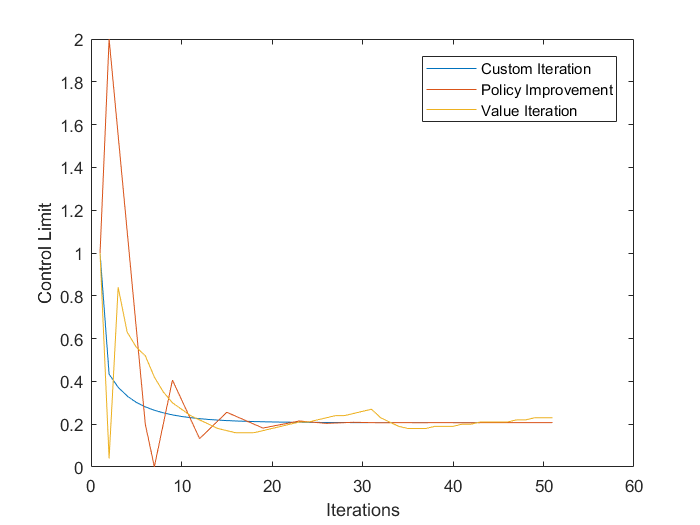
\includegraphics[width=\textwidth]{Plots/CL Weibull2-2 Discount-1 Start-1.png}
\caption{The resulting control limit after each iteration for each algorithm.}
\end{figure}

As you can see, the custom iteration algorithm seems to converge fastest.
Value Iteration seems to perform worst.
As you can see, a problem of Policy Improvement is that it tends to 'overshoot' the optimal policy.
The custom iteration does not have this problem.
We can also repeat this for a Gamma distributed lifetime with shape and rate equal to $2$.
This results in  
\begin{figure}[H]
\centering
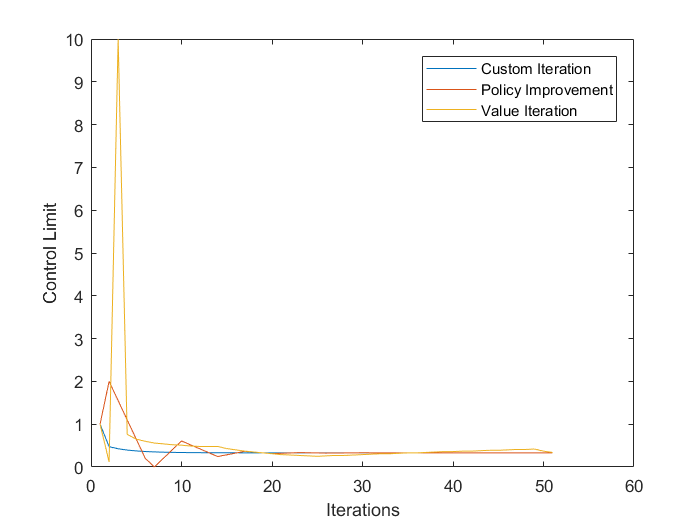
\includegraphics[width=\textwidth]{Plots/CL Gamma2-2 Discount-1 Start-1.png}
\caption{The resulting control limit after each iteration for each algorithm.}
\end{figure}
In this plot, it shows that after 3 iterations, Value Iteration resulted in the policy of never repairing preventively.
The algorithms rank the same on convergence as in the case of the Weibull lifetimes.

\subsection{Other discounts}
If we choose the Weibull distributed lifetime (shape and rate $2$) with the same parameters as in the previous case but with $\beta=2$, we get
\begin{figure}[H]
\centering
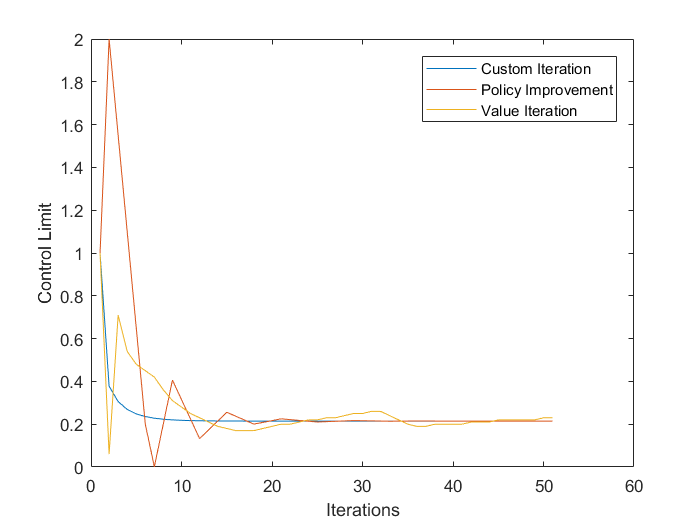
\includegraphics[width=\textwidth]{Plots/CL Weibull2-2 Discount-2 Start-1.png}
\caption{The resulting control limit after each iteration for each algorithm.}
\end{figure}
As you can see this is very much similar to the earlier plots.
Now, changing the discount to $0.5$:
\begin{figure}[H]
\centering
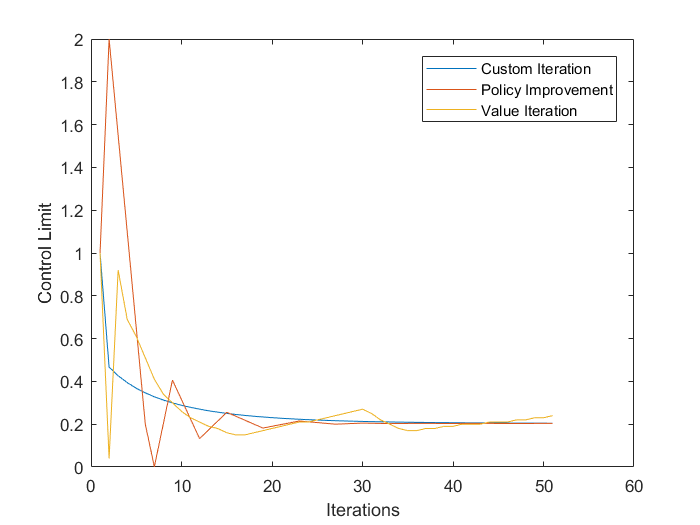
\includegraphics[width=\textwidth]{Plots/CL Weibull2-2 Discount-0.5 Start-1.png}
\caption{The resulting control limit after each iteration for each algorithm.}
\end{figure}
Now the Policy Iteration seems to converge faster or equally as fast as the custom iteration.
\subsection{Other initial control limits}
Choosing the same inputs as the first case but with initial control limit equal to $0.001$:
\begin{figure}[H]
\centering
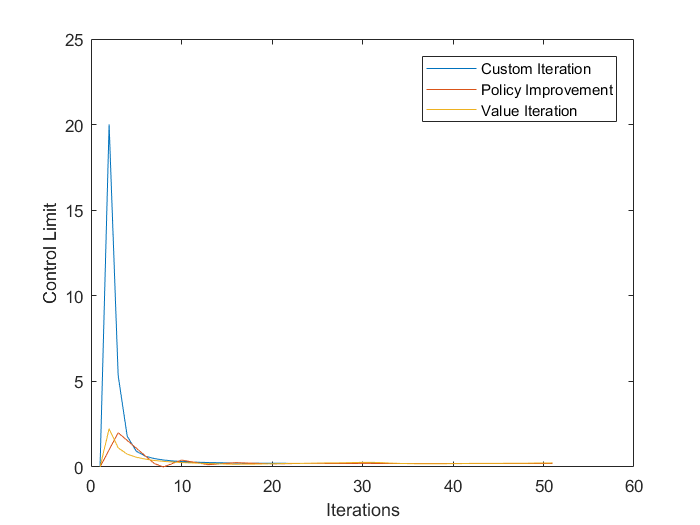
\includegraphics[width=\textwidth]{Plots/CL Weibull2-2 Discount-1 Start-0.001.png}
\caption{The resulting control limit after each iteration for each algorithm.}
\end{figure}
Now the custom iteration seems to converge the slowest of the three.
If we choose an initial control limit equal to $10$, we get
\begin{figure}[H]
\centering
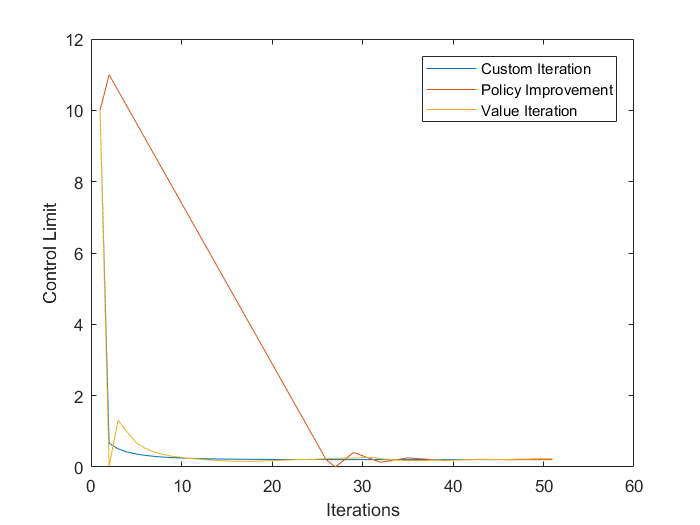
\includegraphics[width=\textwidth]{Plots/CL Weibull2-2 Discount-1 Start-10.png}
\caption{The resulting control limit after each iteration for each algorithm.}
\end{figure}
Now the Policy Iteration clearly converges the slowest, this partially is because it does not increase its step when the improvement step resulted in a lower cost.
This can be seen from the linear decrease between $1$ and $25$.
\subsection{Different costs}
As the only costs in this problem are $c$ and $a$, only their ratio is relevant.
If we choose $a=1$, we get the following plot
\begin{figure}[H]
\centering
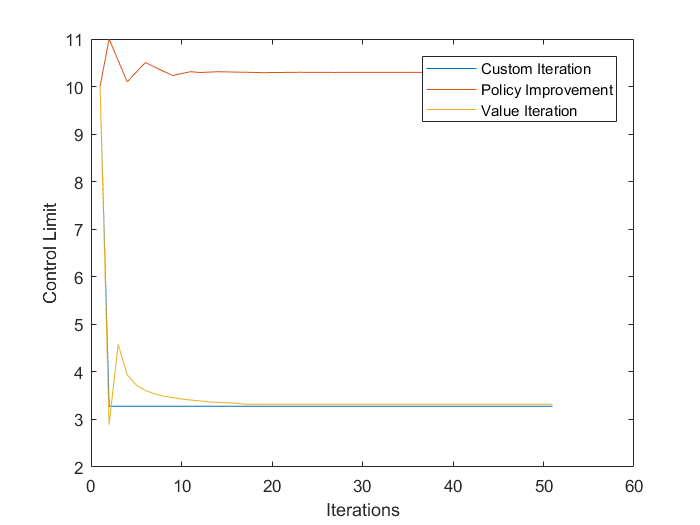
\includegraphics[width=\textwidth]{Plots/CL Weibull2-2 Discount-1 Start-1 a-1.png}
\caption{The resulting control limit after each iteration for each algorithm.}
\end{figure}
In this plot, it is visible that Policy Iteration can get stuck in local optima.
\end{document}